\cleardoublepage

\chapter{Elektrostatikte Sınır Değer Problemleri}

Birçok elektrostatik probleminde, üzerlerinde ya potansiyelin ya da yüzeysel yük yoğunluğunun belirtildiği sınır yüzeyleri yer alır. Green fonksiyonları yöntemini kullanarak, bu tür problemlerin biçimsel çözümlerini 1.10 kesiminde vermiştik. Uygulamaya elverişli durumlarda (ya da uygulamaya elverişli durumlara yapılan soyut yaklaştırmalarda) doğru Green fonksiyonunun bulunması kimi kez kolay kimi kez zordur. Bu nedenle elektrostatikteki sınır değer problemleri için çeşitli yaklaşımlar geliştirilmiştir; bunlardan bazılarının Green fonksiyonları yöntemiyle olan ilişkileri yok denecek kadar azdır. Bu bölümde bu özel tekniklerden şu ikisini inceleyeceğiz: (1) Görüntü yükleri yöntemi. 2) Dik fonksiyonlar cinsinden açılım. Birincisi Green fonksiyonlarının kullanımıyla sıkı sıkıya ilgilidir; ikincisi ise doğrudan doğruya diferansiyel denklem çözmeye dayalı bir yaklaşım olup, Green fonksiyonu kurma yöntemine iyice uzaktır. 

\section{Görüntü Yük Yöntemi}
Görüntü yükleri yöntemi, bir ya da daha fazla noktasal yük ile, örneğin topraklanmış ya da sabit potansiyelde tutulan iletkenler gibi, sınır yüzeyleri kapsayan problemlerde kullanılır. Uygun koşullar altında, problemin geometrisinden esinlenerek, ilgilenilen bölgenin dışına uygun yerlere uygun büyüklükte az sayıda yük yerleştirerek verilen sınır koşullarının aynısını oluşturmak olasıdır. İşte bu yüklere görüntü yükleri ve sınır yüzeyli gerçek problem yerine, sınırların kaldırılarak görüntü yükleriyle genişletilmiş bölgenin konmasına \textbf{görüntü yükleri yöntemi} denir. Görüntü yükleri ilgilenilen hacmin dışında yer almalıdır; çünkü onların potansiyelleri Laplace denkleminin hacim içindeki çözümleri olmalıdır. \textit{Özel integral} (yani Poisson denkleminin çözümü) ise hacmin içindeki gerçek yüklerin potansiyellerinin toplamı ile verilir.

\begin{definition}[Teklik Teoremi]
Bir bölgede verilen bir hacimsel yük yoğunluğu $\rho (x,y,z)$, sınırlar-daki elektriksel potansiyel de $\phi (x,y,z)$ olsun. Bu bölgede elektriksel potansiyeli açıklayan tek bir bir $\phi(x,y,z)$ fonksiyonu vardır. Çözüm tektir.

\ 

\noindent \textbf{I. Teklik Teoremi:} Laplace denkleminin çözümünün tek olduğunu söyler.\\
\textbf{II. Teklik Teoremi:} Birden fazla iletkenin olduğu durumda her bir iletkenin üzerindeki toplam yük verilmişse ve iletkenler arasındaki bölgedeki yük dağılımı biliniyorsa, elektrik alanın değeri tektir.\\
$\therefore$ Şekli ne olursa olsun, içinde boşluk olan bir iletkenin boşluğunda yük yoksa elektrik alanı sıfırdır.
    
\end{definition}

\begin{theorem}
Bizim şimdiye kadar elektrostatikte yaptığımız şeyler aslında hep aynıdır. Verilen problemin şartlarına uygun olarak, elektriksel potansiyeli hangi yöntemle çözebileceğimizi inceledik.

Bir diğer yöntem ise görüntü yök yöntemidir. Bu yöntem de elektriksel potansiyeli bulmak için kullanılan bir yöntemdir. Burada işin püf noktası ne zaman neyi kullanacağımıza dikkat etmek olacaktır. Kendimize, "hangi formülden elektriksel potansiyel kullanırsam bu soruyu ben daha kolay çözerim?" sorusunu sormamız gerekmektedir. Görüntü yük yöntemi, problemi basitleştirmek için orijinal problemin sınır koşullarını sağlayacak uygun yeni bir fiziksel ortam kurmamıza olanak sağlar.\\
\textbf{Jackson:} Basit bir örnek, şekilde görüldüğü gibi, sıfır potansiyelli sonsuz genişlikteki bir iletken düzlemin önünde duran bir noktasal yüktür. Bu gerçek problemin eşdeğerinin, ilk yük ile iletkenin yerinde düşünülen geometrik düzlemin arkasındaki ayna-görüntüsü noktasına konan eşit ve karşıt yüklü problem olduğu açıktır.

Bu şekilde problemi çözmek o kadar kolay değildir. Bunu çözmek yerine, sağda verilen şekil gibi bir ayna simetrisi kuralım. Böylece tam orta noktada topraklanmış iletkenin potansiyeli sıfır olmalıdır. Böylece görüntü yük yöntemine geçmiş oluyoruz.

\begin{center}
\tikzset{every picture/.style={line width=0.75pt}} %set default line width to 0.75pt        

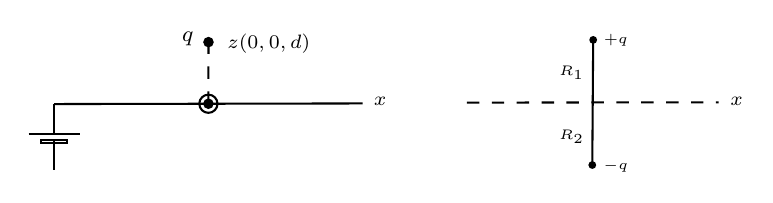
\begin{tikzpicture}[x=0.75pt,y=0.75pt,yscale=-1,xscale=1]
%uncomment if require: \path (0,235); %set diagram left start at 0, and has height of 235

%Shape: Battery [id:dp34859297383687293] 
\draw   (91.15,132.4) -- (91.15,118.14) (78.9,114.97) -- (103.4,114.97) (91.15,114.97) -- (91.15,100.7) (85.02,119.4) -- (85.02,118.14) -- (97.27,118.14) -- (97.27,119.4) -- (85.02,119.4) -- cycle ;
%Straight Lines [id:da07842041091706164] 
\draw    (91.15,100.7) -- (239.8,100.4) ;
\draw [shift={(165.48,100.55)}, rotate = 359.88] [color={rgb, 255:red, 0; green, 0; blue, 0 }  ][fill={rgb, 255:red, 0; green, 0; blue, 0 }  ][line width=0.75]      (0, 0) circle [x radius= 2.01, y radius= 2.01]   ;
%Straight Lines [id:da12973632981107108] 
\draw  [dash pattern={on 4.5pt off 4.5pt}]  (165.48,100.55) -- (165.51,70.86) ;
\draw [shift={(165.51,70.86)}, rotate = 270.08] [color={rgb, 255:red, 0; green, 0; blue, 0 }  ][fill={rgb, 255:red, 0; green, 0; blue, 0 }  ][line width=0.75]      (0, 0) circle [x radius= 2.01, y radius= 2.01]   ;
%Shape: Circle [id:dp5983566304652063] 
\draw   (161.09,100.55) .. controls (161.09,98.13) and (163.05,96.17) .. (165.47,96.17) .. controls (167.9,96.17) and (169.86,98.13) .. (169.86,100.55) .. controls (169.86,102.97) and (167.9,104.93) .. (165.47,104.93) .. controls (163.05,104.93) and (161.09,102.97) .. (161.09,100.55) -- cycle ;
%Straight Lines [id:da46730909892667727] 
\draw  [dash pattern={on 4.5pt off 4.5pt}]  (290,100) -- (411.29,99.86) ;
%Straight Lines [id:da4358326140843938] 
\draw    (350.86,69.79) -- (350.5,119.69) -- (350.43,130.07) ;
\draw [shift={(350.43,130.07)}, rotate = 90.41] [color={rgb, 255:red, 0; green, 0; blue, 0 }  ][fill={rgb, 255:red, 0; green, 0; blue, 0 }  ][line width=0.75]      (0, 0) circle [x radius= 1.34, y radius= 1.34]   ;
\draw [shift={(350.86,69.79)}, rotate = 90.41] [color={rgb, 255:red, 0; green, 0; blue, 0 }  ][fill={rgb, 255:red, 0; green, 0; blue, 0 }  ][line width=0.75]      (0, 0) circle [x radius= 1.34, y radius= 1.34]   ;

% Text Node
\draw (151.37,64.4) node [anchor=north west][inner sep=0.75pt]  [font=\footnotesize]  {$q$};
% Text Node
\draw (243.66,96) node [anchor=north west][inner sep=0.75pt]  [font=\scriptsize]  {$x$};
% Text Node
\draw (173.14,65.26) node [anchor=north west][inner sep=0.75pt]  [font=\scriptsize]  {$z( 0,0,d)$};
% Text Node
\draw (354.57,65.54) node [anchor=north west][inner sep=0.75pt]  [font=\tiny]  {$+q$};
% Text Node
\draw (354.29,126.4) node [anchor=north west][inner sep=0.75pt]  [font=\tiny]  {$-q$};
% Text Node
\draw (415.43,96) node [anchor=north west][inner sep=0.75pt]  [font=\scriptsize]  {$x$};
% Text Node
\draw (333,80.97) node [anchor=north west][inner sep=0.75pt]  [font=\tiny]  {$R_{1}$};
% Text Node
\draw (333,111.54) node [anchor=north west][inner sep=0.75pt]  [font=\tiny]  {$R_{2}$};

\draw [draw opacity=0]  (89.15,100.7) -- (93.15,100.7)(91.15,98.7) -- (91.15,102.7) ;
\end{tikzpicture}
\end{center}

Burada yüzey yükünden kaynaklanan bir katkı daha vardır. Topraklasak bile burada, $\rho_{s}$ yüzey yükünden kaynaklanan bir katkı daha vardır çünkü bütün yükleri toplamamız gerekmektedir.
\[ V(x,y,z) = \dfrac{k q}{\sqrt{x^{2} + y^{2} + (z-d)^{2}}}  + k \int_{S} \dfrac{\rho_{s}}{R_{1}} ds \]
\[ V = k \dfrac{q}{R_{1}} + \dfrac{k(-q)}{R_{2}} \]
Bu sonuç, sınır koşulunun sağlandığı durumda ortaya çıkmaktadır. Bu durumda çözüm tektir diyerek ayna simetrisini kullanabiliriz.\\
$\therefore$ Görüntü yük her zaman gerçek yükün zıt işaretlisi olmalıdır.\\
$\therefore$ Elektriksel potansiyel gerçek yükün ve görüntü yükün dışında bir noktada bulunur.\\
$\therefore$ Görüntü yükün varlığından kaynaklanan yüke indüklenmiş yüzey yükü denir.

\

İndüklenmiş yüzey yükünü bulalım. İletkenin hemen dışında elektrik alan,
\[ \Vec{E} = \dfrac{\sigma}{\varepsilon_{0}} \hat{n}  \quad \Vec{E} = - \dfrac{\partial \phi}{\partial n} \hat{n} \]
\[ \hat{a}_{n} \rightarrow \hat{a}_{z} \Rightarrow \sigma = \varepsilon_{0} E_{z} = - \varepsilon_{0} \dfrac{\partial \phi}{\partial z} \Bigg|_{z=0} \]
İncelediğimiz problemde uzaklığı $d$ alarak yerine koyalım,
\[ V (x,y,z) = \dfrac{kq}{\sqrt{x^{2} + y^{2} + (z-d)^{2}}} + \dfrac{k (-q)}{\sqrt{x^{2} + y^{2} + (z+d)^{2}}} \]
$z=0$'da indüklenmiş yüzey yükünü bulalım,
\[ \sigma = - \varepsilon_{0} \dfrac{\partial \phi}{\partial z} \Bigg|_{z=0}  \]
İlk olarak kısmi türevi alarak yerine koyalım,
\[ x^{2} + y^{2} = r^{2} \textrm{ için} \]
\[ \dfrac{\partial \phi}{\partial z} \Bigg|_{z=0} =  \dfrac{\partial}{\partial z}  \Bigg\{ \dfrac{1}{4 \pi \varepsilon_{0}} \dfrac{q}{\sqrt{r^{2} + (z-d)^{2}}} + \dfrac{1}{4 \pi \varepsilon_{0}} \dfrac{ (-q)}{\sqrt{r^{2} + (z+d)^{2}}}  \Bigg\} \]
\[ =   \dfrac{q}{4 \pi \varepsilon_{0}} \dfrac{\partial}{\partial z}  \Bigg\{ \dfrac{1}{\sqrt{r^{2} + (z-d)^{2}}} - \dfrac{1}{\sqrt{r^{2} + (z+d)^{2}}}  \Bigg\} \]
\[ = \dfrac{q}{4 \pi \varepsilon_{0}} \dfrac{\partial}{\partial z}  \Bigg\{ (r^{2} + (z-d)^{2})^{-1/2} - (r^{2} + (z+d)^{2})^{-1/2} \Bigg\} \]
\begin{align*}
&= \dfrac{q}{4 \pi \varepsilon_{0}}  \Bigg\{ \Big[ - \dfrac{1}{2} (r^{2} + (z-d)^{2})^{-3/2} 2(z-d) (1) \Big] \\
&- \Big[ - \dfrac{1}{2} (r^{2} + (z+d)^{2})^{-3/2} 2(z+d) (1) \Big]  \Bigg\}
\end{align*}
\begin{align*}
&= \dfrac{q}{4 \pi \varepsilon_{0}}  \Bigg\{ \Big[ -  (r^{2} + (z-d)^{2})^{-3/2} (z-d)  \Big] \\
& + \Big[  (r^{2} + (z+d)^{2})^{-3/2} (z+d) \Big]  \Bigg\}
\end{align*}
\[ = \dfrac{q}{4 \pi \varepsilon_{0}}  \Bigg\{ - \dfrac{(z-d)}{ (r^{2} + (z-d)^{2})^{3/2}} + \dfrac{(z+d)}{ (r^{2} + (z+d)^{2})^{3/2}}  \Bigg\} \Bigg|_{z=0} \]
\[ = \dfrac{q}{4 \pi \varepsilon_{0}}  \Bigg\{ - \dfrac{(-d)}{ (r^{2} + (-d)^{2})^{3/2}} + \dfrac{(d)}{ (r^{2} + (d)^{2})^{3/2}}  \Bigg\} \]
\[ = \dfrac{q}{4 \pi \varepsilon_{0}}  \Bigg\{  \dfrac{d}{ (r^{2} + d^{2})^{3/2}} + \dfrac{d}{ (r^{2} + d^{2})^{3/2}}  \Bigg\} \]
\[ \dfrac{\partial \phi}{\partial z} \Bigg|_{z=0}  = \dfrac{q}{4 \pi \varepsilon_{0}}  \Bigg\{  \dfrac{2 d}{ (r^{2} + d^{2})^{3/2}} \Bigg\} \]
\[ \sigma = - \varepsilon_{0} \dfrac{\partial \phi}{\partial z} \Bigg|_{z=0} = - \cancel{\varepsilon_{0}}  \dfrac{q}{4 \pi \cancel{\varepsilon_{0}}}  \Bigg\{  \dfrac{\cancel{2} d}{ (r^{2} + d^{2})^{3/2}} \Bigg\}  \]
\[ \sigma = - \dfrac{q}{2 \pi} \dfrac{d}{(r^{2} + d^{2})^{3/2}} \]
Sistemin toplam Q yükünü bulalım,
\[Q_{\textrm{toplam}} = \int \sigma da \]
\[ Q = \int_{0}^{\infty} \int_{0}^{2 \pi} \sigma r dr d\theta dr \]
\[ Q = \int_{0}^{\infty} \int_{0}^{2 \pi} \Big\{  - \dfrac{q}{2 \pi} \dfrac{d}{(r^{2} + d^{2})^{3/2}} \Big\} r d\theta dr \]
\[ Q = \int_{0}^{\infty} \Big\{  - \dfrac{q}{2 \pi} \dfrac{d}{(r^{2} + d^{2})^{3/2}} \Big\} r  dr  \int_{0}^{2 \pi} d\theta \]
\[ Q = - \dfrac{qd}{\cancel{2 \pi}} \cancel{ \big( 2 \pi \big)} \underbrace{\int_{0}^{\infty} \Big\{ \dfrac{1}{(r^{2} + d^{2})^{3/2}} \Big\} r  dr}_{I}  \]
\[ \Rightarrow I = \int \Big\{ \dfrac{1}{(r^{2} + d^{2})^{3/2}} \Big\} r  dr \]
\[ u = r^{2} + d^{2} \rightarrow \dfrac{du}{dr} = 2r \rightarrow du = 2r dr \]
\[ I =  \begingroup \color{red} \dfrac{1}{2} \endgroup \int \Big\{ \dfrac{1}{(r^{2} + d^{2})^{3/2}} \Big\}  \begingroup \color{red}2 \endgroup r  dr \]
Böylece,
\[ I =  \begingroup \color{red} \dfrac{1}{2} \endgroup \int \dfrac{1}{u^{3/2}} du =\begingroup \color{red} \dfrac{1}{2} \endgroup \dfrac{u^{-1/2}}{-\dfrac{1}{2}} = \begingroup \color{red} \dfrac{1}{2} \endgroup  ( - \dfrac{2}{\sqrt{u}} ) = - \dfrac{1}{\sqrt{u}} \]
\[  u = r^{2} + d^{2} \textrm{ yerine yazılırsa,} \]
\[ \Rightarrow I = - \dfrac{1}{\sqrt{r{2} + d^{2}}} \]
\[ Q = - qd \Big\{ - \dfrac{1}{\sqrt{r^{2} + d^{2}}} \Big\} \Bigg|^{\infty}_{0} \]
\[ Q = - qd \Big\{ \cancelto{0}{- \dfrac{1}{\sqrt{\infty^{2} + d^{2}}}} +  \dfrac{1}{\sqrt{d^{2}}} \Big\} = - q \cancel{\dfrac{d}{d}} = -q\]
\end{theorem}

\section{Topraklanmış İletken Küre ve Nokta Yük Problemi}
\begin{theorem}

\ 

\begin{center}
\tikzset{every picture/.style={line width=0.75pt}} %set default line width to 0.75pt        
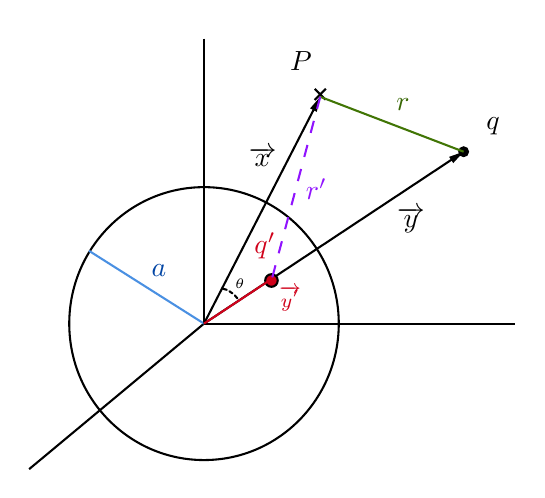
\begin{tikzpicture}[x=0.75pt,y=0.75pt,yscale=-1,xscale=1]
%uncomment if require: \path (0,438); %set diagram left start at 0, and has height of 438

%Straight Lines [id:da3363021434624792] 
\draw    (184.46,142.75) -- (184.46,228.65) -- (184.46,280.08) ;
%Straight Lines [id:da9829878340854751] 
\draw    (184.46,280.08) -- (334.5,280.08) ;
%Straight Lines [id:da8021753493849154] 
\draw    (184.46,280.08) -- (100.2,350.2) ;
%Shape: Ellipse [id:dp3387390173452981] 
\draw   (119.53,280.08) .. controls (119.53,243.77) and (148.6,214.33) .. (184.46,214.33) .. controls (220.31,214.33) and (249.38,243.77) .. (249.38,280.08) .. controls (249.38,316.38) and (220.31,345.82) .. (184.46,345.82) .. controls (148.6,345.82) and (119.53,316.38) .. (119.53,280.08) -- cycle ;
%Straight Lines [id:da9624418256546885] 
\draw [color={rgb, 255:red, 74; green, 144; blue, 226 }  ,draw opacity=1 ]   (184.46,280.08) -- (129.05,245.01) ;
%Straight Lines [id:da35498645246042104] 
\draw    (100,138) ;
\draw   (237.86,166.99) -- (243.07,172.23)(243.16,166.89) -- (237.77,172.32) ;
%Shape: Ellipse [id:dp24063798072870257] 
\draw  [fill={rgb, 255:red, 0; green, 0; blue, 0 }  ,fill opacity=1 ] (307.45,197.26) .. controls (307.45,198.43) and (308.39,199.38) .. (309.55,199.38) .. controls (310.71,199.38) and (311.65,198.43) .. (311.65,197.26) .. controls (311.65,196.09) and (310.71,195.14) .. (309.55,195.14) .. controls (308.39,195.14) and (307.45,196.09) .. (307.45,197.26) -- cycle ;
%Straight Lines [id:da3344035038325499] 
\draw    (239.55,172.58) -- (184.46,280.08) ;
\draw [shift={(240.46,170.8)}, rotate = 117.14] [fill={rgb, 255:red, 0; green, 0; blue, 0 }  ][line width=0.08]  [draw opacity=0] (7.2,-1.8) -- (0,0) -- (7.2,1.8) -- cycle    ;
%Straight Lines [id:da5576504295503066] 
\draw    (307.88,198.36) -- (184.46,280.08) ;
\draw [shift={(309.55,197.26)}, rotate = 146.49] [fill={rgb, 255:red, 0; green, 0; blue, 0 }  ][line width=0.08]  [draw opacity=0] (7.2,-1.8) -- (0,0) -- (7.2,1.8) -- cycle    ;
%Shape: Ellipse [id:dp44088406147683445] 
\draw  [fill={rgb, 255:red, 208; green, 2; blue, 27 }  ,fill opacity=1 ] (213.94,259.31) .. controls (213.94,260.99) and (215.29,262.35) .. (216.96,262.35) .. controls (218.62,262.35) and (219.98,260.99) .. (219.98,259.31) .. controls (219.98,257.63) and (218.62,256.27) .. (216.96,256.27) .. controls (215.29,256.27) and (213.94,257.63) .. (213.94,259.31) -- cycle ;
%Straight Lines [id:da4540267103867084] 
\draw [color={rgb, 255:red, 208; green, 2; blue, 27 }  ,draw opacity=1 ]   (184.46,280.08) -- (215.72,259.44) ;
%Straight Lines [id:da5460132362031128] 
\draw [color={rgb, 255:red, 65; green, 117; blue, 5 }  ,draw opacity=1 ]   (240.46,170.8) -- (309.55,197.26) ;
%Straight Lines [id:da021801983615440057] 
\draw [color={rgb, 255:red, 144; green, 19; blue, 254 }  ,draw opacity=1 ] [dash pattern={on 4.5pt off 4.5pt}]  (240.46,170.8) -- (216.96,259.31) ;
%Shape: Free Drawing [id:dp38355535695344223] 
\draw  [line width=0.75] [line join = round][line cap = round] (193.43,263.21) .. controls (193.48,263.26) and (193.52,263.31) .. (193.57,263.36) ;
%Shape: Free Drawing [id:dp9355411290145775] 
\draw  [line width=0.75] [line join = round][line cap = round] (193.86,263.36) .. controls (194.38,263.5) and (194.9,263.64) .. (195.43,263.79) ;
%Shape: Free Drawing [id:dp04832018266107674] 
\draw  [line width=0.75] [line join = round][line cap = round] (196.71,264.5) .. controls (197.19,264.83) and (197.67,265.17) .. (198.14,265.5) ;
%Shape: Free Drawing [id:dp4041626764172217] 
\draw  [line width=0.75] [line join = round][line cap = round] (199.29,266.5) .. controls (199.71,266.98) and (200.14,267.45) .. (200.57,267.93) ;

% Text Node
\draw (224.48,147.59) node [anchor=north west][inner sep=0.75pt]    {$P$};
% Text Node
\draw (319.04,179.34) node [anchor=north west][inner sep=0.75pt]    {$q$};
% Text Node
\draw (204.52,193.69) node [anchor=north west][inner sep=0.75pt]    {$\overrightarrow{x}$};
% Text Node
\draw (275.97,222.79) node [anchor=north west][inner sep=0.75pt]    {$\overrightarrow{y}$};
% Text Node
\draw (207.27,234.56) node [anchor=north west][inner sep=0.75pt]  [color={rgb, 255:red, 208; green, 2; blue, 27 }  ,opacity=1 ]  {$q'$};
% Text Node
\draw (219.36,260.25) node [anchor=north west][inner sep=0.75pt]  [font=\scriptsize,color={rgb, 255:red, 208; green, 2; blue, 27 }  ,opacity=1 ]  {$\overrightarrow{y'}$};
% Text Node
\draw (275.6,170) node [anchor=north west][inner sep=0.75pt]  [color={rgb, 255:red, 56; green, 103; blue, 4 }  ,opacity=1 ]  {$r$};
% Text Node
\draw (232,208.8) node [anchor=north west][inner sep=0.75pt]  [color={rgb, 255:red, 144; green, 19; blue, 254 }  ,opacity=1 ]  {$r'$};
% Text Node
\draw (157.77,250) node [anchor=north west][inner sep=0.75pt]  [color={rgb, 255:red, 2; green, 69; blue, 164 }  ,opacity=1 ]  {$a$};
% Text Node
\draw (197.86,257.26) node [anchor=north west][inner sep=0.75pt]  [font=\tiny]  {$\theta $};
\end{tikzpicture}
\captionof*{figure}{$a$ yarıçaplı iletken küre karşısında $q$ yükü ve $q'$ görüntü yükü.}
\end{center}
 
  Görüntü yükleri problemini açıklamak için, şekilde verilmiş a yarıçaplı topraklanmış bir iletken kürenin karşısına merkezden $\Vec{y}$ uzaklığına konmuş noktasal q yükü problemini ele alalım. $\phi (|\Vec{x}| = a) = 0 $ olacak şekilde $\phi (\Vec{x})$ potansiyelini arıyoruz. Simetri nedeniyle $q'$ görüntü yükünün (sadece bir tek görüntü yükünün gerekli olduğunu varsayıyoruz) başlangıçtan $q$ yüküne uzanan ışın üzerinde olacağı açıktır. $q$ yükünün küre dışında bulunduğunu varsayarsak, $\Vec{y}'$ görüntü yeri küre içinde olacaktır. $q$ ve $q'$ yüklerince oluşturulan potansiyeli yazalım [\textbf{Jackson}]. 
\[ q' \rightarrow \textrm{ görüntü yükü} \]
\[ q \rightarrow \Vec{y} + \Vec{r} = \Vec{x} \Rightarrow \Vec{r} = \Vec{x} - \Vec{y} \]
\[ q' \rightarrow \Vec{y'} + \Vec{r'} = \Vec{x} \Rightarrow \Vec{r'} = \Vec{x} - \Vec{y'} \]
\[ \Vec{x} = x \hat{n} \quad \Vec{y} = y \hat{n}' \]
$q'$ ve $y'$ öyle olmalı ki $|\Vec{x}| = a$'da potansiyel sıfır.
\[\phi (\Vec{x}) = \dfrac{kq}{|\Vec{x} - \Vec{y}|} + \dfrac{kq'}{|\Vec{x} - \Vec{y'}|} = \dfrac{kq}{|x \hat{n} - y \hat{n}'|} + \dfrac{kq'}{|x\hat{n} - y' \hat{n}'|} \tag{2.1}\]
\[\phi (\Vec{x})  = k \Big\{ \dfrac{q}{|x \hat{n} - y \hat{n}'|} + \dfrac{q'}{|x\hat{n} - y' \hat{n}'|} \Big\} \tag{2.2}\]
Daha sonra kolaylık olması için, birinci terimde $x$'i, ikinci terimde $y'$'nü mutlak değer işaretinin dışarısına çıkartalım,
\[\phi (\Vec{x})  = k \Bigg\{ \dfrac{q}{ x | \hat{n} - \dfrac{y}{x} \hat{n}'|} + \dfrac{q'}{ y' |\dfrac{x}{y'}\hat{n} - \hat{n}'|} \Bigg\} \]
\[\phi (x=a)  = k \Bigg\{ \dfrac{q}{ a | \hat{n} - \dfrac{y}{a} \hat{n}'|} + \dfrac{q'}{ y' |\dfrac{a}{y'}\hat{n} - \hat{n}'|} \Bigg\} = 0 \]
Bu potansiyeli şu şekilde yazalım,
\[\phi (x=a)  = k \Bigg\{ \dfrac{q}{ a | \hat{n} - \dfrac{y}{a} \hat{n}'|} + \dfrac{q'}{ y' |\hat{n}' - \dfrac{a}{y'}\hat{n}'|} \Bigg\} = 0 \tag{2.3}\]
Burada büyüklük olarak yazdığımız için 2. terimde yaptığımız değişiklik herhangi bir şeyi etkilememektedir.
\[ 0 = \begingroup \color{red} \dfrac{q}{a} \endgroup \dfrac{k}{  | \hat{n} - \begingroup \color{blue} \dfrac{y}{a} \endgroup \hat{n}'|} + \begingroup \color{red} \dfrac{q'}{y'} \endgroup \dfrac{k}{|  \hat{n}' -\begingroup \color{blue} \dfrac{a}{y'} \endgroup \hat{n}|} \]
Bu ifadenin $0$'a eşit olabilmesi için,
\[ \begingroup \color{red} \dfrac{q}{a} = - \dfrac{-q'}{y'} \endgroup \textrm{ ve }  \begingroup \color{blue} \dfrac{y}{a} = \dfrac{a}{y'}  \endgroup \]
olmalıdır. Bu eşitliklerin seçimi $\hat{n} \cdot \hat{n}'$'nün her değeri için $\phi (x=a) = 0$ yapacaktır. Bu durumda görüntü yükünün büyüklüğü ve yeri,
\[ q' = - \dfrac{q}{a} y' = - \dfrac{q}{a} (\dfrac{a^{2}}{y}) = - \dfrac{qa}{y} \]
\[ q'=  - \dfrac{qa}{y} \quad y'= \dfrac{a^{2}}{y} \]
şeklinde yazılabilir. q yükü küreye yaklaştıkça, görüntü yükünün mutlak değerce büyüdüğüne ve merkezden dışa doğru uzaklaştığına dikkat ediniz. q yükü, küre yüzeyinin hemen dışında ise, görüntü yükü buna eşit ve karşıt işaretli olup yüzeyin hemen içindedir. Görüntü yükünü hesapladığımıza göre, artık topraklanmış iletken küre dışında duran q yükü biçimindeki esas problemimize dönebilir ve çeşitli etkileri ele alabiliriz [\textbf{Jackson}]. \\
İndüklenmiş yüzey yükünü bulmamız gerekiyor. Görüntü yük varlığından kaynaklanan kürenin yüzeyi üzerinde bulunan yük yoğunluğunu bulalım. $\phi (\Vec{x})$'i yazıp, türevini alıp $\sigma$ yük yoğunluğunu hesaplayacağız.
\[ |\Vec{x} - \Vec{y}| = \sqrt{x^{2} + y^{2} - 2 xy \cos \theta} \]
\[ \phi (x) = \dfrac{kq}{\bigg\{  x^{2} + y^{2} - 2xy \cos \theta  \bigg\}^{1/2} } + \dfrac{kq'}{\bigg\{  x^{2} + y'^{2} - 2xy' \cos \theta  \bigg\}^{1/2} } \]
\begin{align*}
 \dfrac{\partial \phi (x)}{\partial x} &= kq (-\dfrac{1}{\cancel{2}}) \Big\{ x^{2} + y^{2} - 2xy \cos \theta \Big\}^{-3/2} (\cancel{2}x - \cancel{2}y \cos \theta)\\ 
 &+ k q' (-\dfrac{1}{\cancel{2}})  \Big\{ x^{2} + y'^{2} - 2xy' \cos \theta \Big\}^{-3/2} (\cancel{2}x - \cancel{2}y' \cos \theta)
\end{align*}
\begin{align*}
 \dfrac{\partial \phi (x)}{\partial x} &= kq  \Big\{ x^{2} + y^{2} - 2xy \cos \theta \Big\}^{-3/2} (-x + y \cos \theta)\\ 
 &+ k q'  \Big\{ x^{2} + y'^{2} - 2xy' \cos \theta \Big\}^{-3/2} (-x + y' \cos \theta)
\end{align*}
\newpage
\begin{align*}
 \dfrac{\partial \phi (x)}{\partial x} \Bigg|_{x=a} &= kq \Big\{ a^{2} + y^{2} - 2ay \cos \theta \Big\}^{-3/2} ( y \cos \theta -a )\\ 
 &+ k q' \Big\{ a^{2} + y'^{2} - 2ay' \cos \theta \Big\}^{-3/2} (y' \cos \theta - a)
\end{align*}
Burada $q'$ ve $y'$ terimlerini yerine yazalım,
\begin{align*}
 \dfrac{\partial \phi (x)}{\partial x} \Bigg|_{x=a} &= kq \Big\{ a^{2} + y^{2} - 2ay \cos \theta \Big\}^{-3/2} ( y \cos \theta -a )\\ 
 &+ k ( - \dfrac{qa}{y}) \Big\{ a^{2} + (\dfrac{a^{2}}{y})^{2} - 2x(\dfrac{a^{2}}{y}) \cos \theta \Big\}^{-3/2} ((\dfrac{a^{2}}{y}) \cos \theta - a)
\end{align*}
\[ \dfrac{\partial \phi (x)}{\partial x} \Bigg|_{x=a} = \dfrac{kq ( y \cos \theta -a ) }{\Big\{ a^{2} + y^{2} - 2ay \cos \theta \Big\}^{3/2}} - k q \dfrac{a}{y} \dfrac{(\dfrac{a^{2}}{y} \cos \theta - a)}{ \Big\{ a^{2} + \dfrac{a^{4}}{y^{2}}- 2 \dfrac{a^{3}}{y} \cos \theta \Big\}^{3/2}}  \]
Burada sadeleştirme işlemi yapabilmek için 2. terimi düzenleyelim,
\[  \Rightarrow \dfrac{a}{y} \dfrac{(\dfrac{a^{2}}{y} \cos \theta - a)}{ \Big\{ \begingroup \color{red}  \dfrac{a^{2}}{y^{2}} \endgroup \Big[ y^{2} + a^{2} - 2 a y \cos \theta \Big] \Big\}^{3/2}} = \dfrac{ \dfrac{a}{y}  \begingroup \color{red}  \dfrac{y^{3}}{a^{3}} \endgroup (\dfrac{a^{2}}{y} \cos \theta - a)}{ \Big\{ y^{2} + a^{2} - 2 a y \cos \theta \Big\}^{3/2}}  \]
\[  \Rightarrow = \dfrac{  \begingroup \color{red}  \dfrac{y^{2}}{a^{2}} \endgroup (\dfrac{a^{2}}{y} \cos \theta - a)}{ \Big\{  y^{2} + a^{2} - 2 a y \cos \theta \Big\}^{3/2}} =\dfrac{ ( y \cos \theta - \dfrac{y^{2}}{a})}{ \Big\{  y^{2} + a^{2} - 2 a y \cos \theta \Big\}^{3/2}} \]
Düzenledikten sonra tekrar $\phi(x)$'de yerine yazarsak,
\[ \dfrac{\partial \phi (x)}{\partial x} \Bigg|_{x=a} = \dfrac{kq ( y \cos \theta -a ) }{\Big\{ a^{2} + y^{2} - 2ay \cos \theta \Big\}^{3/2}} - k q \dfrac{ ( y \cos \theta - \dfrac{y^{2}}{a})}{ \Big\{  y^{2} + a^{2} - 2 a y \cos \theta \Big\}^{3/2}} \]
\[ \dfrac{\partial \phi (x)}{\partial x} \Bigg|_{x=a} = \dfrac{kq ( \dfrac{y^{2}}{a} -a ) }{\Big\{ a^{2} + y^{2} - 2ay \cos \theta \Big\}^{3/2}} = \dfrac{kq}{a}  \dfrac{( y^{2} -a^{2} ) }{\Big\{ a^{2} + y^{2} - 2ay \cos \theta \Big\}^{3/2}}  \]
\[ \dfrac{\partial \phi (x)}{\partial x} \Bigg|_{x=a} = \dfrac{kq}{a}  \dfrac{( y^{2} -a^{2} ) }{\Big\{ a^{2} + y^{2} - 2ay \cos \theta \Big\}^{3/2}} = \dfrac{kq}{a}  \dfrac{y^{2} ( 1 - \dfrac{a^{2}}{y^{2}}) }{\Big\{ \begingroup \color{red} y^{2} \endgroup  \Big[ \dfrac{a^{2}}{y^{2}} + 1 - \dfrac{2a}{y} \cos \theta \Big] \Big\}^{3/2}}  \]
\[ \dfrac{\partial \phi (x)}{\partial x} \Bigg|_{x=a} = \dfrac{kq}{a}  \dfrac{y^{2} ( 1 - \dfrac{a^{2}}{y^{2}}) }{\Big\{ \begingroup \color{red} y^{2} \endgroup \Big[ \dfrac{a^{2}}{y^{2}} + 1 - \dfrac{2a}{y} \cos \theta \Big] \Big\}^{3/2}} =  \dfrac{kq}{a}  \begingroup \color{red} \dfrac{1}{y^{3}} \endgroup \dfrac{y^{2} ( 1 - \dfrac{a^{2}}{y^{2}}) }{\Big\{ \dfrac{a^{2}}{y^{2}} + 1 - \dfrac{2a}{y} \cos \theta \Big\}^{3/2}} \]
Denklemi $a$ ile çarpıp bölersek,
\[ \dfrac{\partial \phi (x)}{\partial x} \Bigg|_{x=a} =  \dfrac{kq}{a^{2}}  \dfrac{a}{y}  ( 1 - \dfrac{a^{2}}{y^{2}}) \dfrac{1}{\Big\{ \dfrac{a^{2}}{y^{2}} + 1 - \dfrac{2a}{y} \cos \theta \Big\}^{3/2}}  \]
\[ \sigma = - \varepsilon_{0} \dfrac{\partial \phi}{\partial x} \Bigg|_{x=a} = - \cancel{\varepsilon_{0}}  \dfrac{1}{4 \pi \cancel{\varepsilon_{0}}}  \dfrac{q}{a^{2}}  \dfrac{a}{y}  ( 1 - \dfrac{a^{2}}{y^{2}}) \dfrac{1}{\Big\{ \dfrac{a^{2}}{y^{2}} + 1 - \dfrac{2a}{y} \cos \theta \Big\}^{3/2}}   \]
\[ \sigma = - \dfrac{1}{4 \pi}  \dfrac{q}{a^{2}}  \dfrac{a}{y}  ( 1 - \dfrac{a^{2}}{y^{2}}) \dfrac{1}{\Big\{ \dfrac{a^{2}}{y^{2}} + 1 - \dfrac{2a}{y} \cos \theta \Big\}^{3/2}} \tag{2.5} \]
q yükünü etkiyen kuvveti hesaplayalım. En kolay yol $q$ yüküyle $q'$ görüntü yükü arasındaki kuvveti yazmaktır. Aralarındaki uzaklık $y-y' = y (1- a^{2}/y^{2})$'dir. Dolayısıyla Coulomb yasasına göre, bu çekici kuvveti yazalım,
\[y-y' = y - \dfrac{a^{2}}{y} = y (1-\dfrac{a^{2}}{y^{2}}) \]
\[ |\Vec{F}| = k \dfrac{qq'}{\big\{ y (1- \dfrac{a^{2}}{y^{2}})  \big\}^{2}}  = \dfrac{kq (- \dfrac{qa}{y})}{y^{2} \big(1 - \dfrac{a^{2}}{y^{2}} \big)^{2}} \]
Denklemi $a^{2}$ ile çarpıp bölersek,
\[ |\Vec{F}| = - k \dfrac{q^{2}}{a^{2}} (\dfrac{a^{3}}{y^{3}}) \dfrac{1}{ \big(1 - \dfrac{a^{2}}{y^{2}}\big)^{2}} \tag{2.6}\]
$y \gg a$ için,
\[ |\Vec{F}| = - k \dfrac{q^{2}}{a^{2}} (\dfrac{a^{3}}{y^{3}}) \dfrac{1}{\big(1 - \cancel{\dfrac{a^{2}}{y^{2}}} \big)^{2}} \]
\[ |\Vec{F}| = -k \dfrac{q^{2}}{a^{2}} \dfrac{a^{3}}{y^{3}} = -k q^{2} \dfrac{a}{y^{3}} \]
\dangersign \ Burada büyüklük olduğu için $-$ işareti olmayacak ama yükün işaretini göz önüne alarak koymuş olalım ki çekici bir kuvvet olduğunu görelim.
\end{theorem}

\ 

Bu kuvvet, büyük aralıklar için ters küp yasasıdır; fakat küreye yakın durumlarda, küre yüzeyinden olan uzaklığın karesiyle ters orantılıdır.\\
Tüm tartışma, küre dışındaki noktasal q yükü varsayımına dayandırıldı. Gerçekte sonuçlarımızı olduğu gibi küre içindeki $q$ yükü haline de uygulayabiliriz. Gerekli tek değişiklik Denklem (2.5)'teki yüzeysel yük yoğunluğunda ortaya çıkar. İletkenden dışa doğru olan dik türev bu kez içeriye doğru olup bir işaret değişikliği getirir. Bu durumda $y \leq a $ olduğunu gözönünde tutarak tüm formüllerin aynısını kopya edebilir.

 
\section{Yalıtılmış İletken Küre ve Nokta Yük Problemi}

Önceki kısımda topraklanmış bir küre karşısında noktasal $q$ yükü problemini ele almış ve küre üzerinde bir yüzeysel yük yoğunluğu oluşturduğunu görmüştük. Bu yükün toplamı $q' = -aq/y$ idi ve tüm kuvvetlerin etkisi altında dengece olacak biçimde yüzey üzerine dağılmıştı.

\ 

Eğer üzerinde toplam Q yükü bulunduran yalıtılmış bir iletken küre karşısında noktasal $q$ yükü problemini ele alırsak, potansiyeli çizgisel üst üste binme ilkesi yardımıyla bulabiliriz. İşlemsel anlamda, üzerinde yüzeyine dağılmış $q'$ yükü bulunan topraklanmış iletken küre ile başlarız. Sonra topraklama telini kesip küre üzerine $(Q-q')$ kadar yük ekleriz. Bu, küre üzeridneki toplam yükü $Q$'ya çıkarır. Potansiyelini bulmak için şuna dikkat etmemiz yeter: $q$ noktasal yüküyle ilgili elektrostatik kuvvetler $q'$ yükü tarafından dengelendiklerinden, eklenen $(Q-q')$ yükü yüzey üzerinde düzgün olarak dağılacaktır. Dolayısıyla eklenen bu $(Q-q')$ yükünün potansiyeli, en azından küre dışındaki noktalar için, merkeze konan aynı büyüklükteki noktasal bir yükün potansiyeliyle aynı olacaktır.

\newpage

\begin{theorem}
İletken küreyi topraklayalım. Topraklanmış kürenin yükü $q'$ olsun. Kürenin toprak hattını keselim ve küreye $(Q-q')$ kadar yük ekleyelim. $\phi_{p}=?$
\begin{center}
\tikzset{every picture/.style={line width=0.75pt}} %set default line width to 0.75pt        
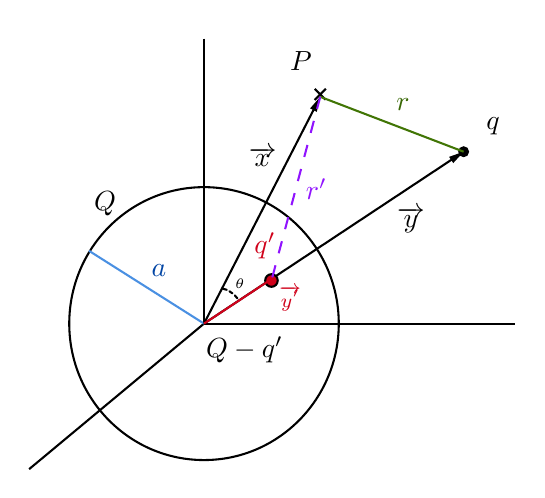
\begin{tikzpicture}[x=0.75pt,y=0.75pt,yscale=-1,xscale=1]
%uncomment if require: \path (0,438); %set diagram left start at 0, and has height of 438

%Straight Lines [id:da3363021434624792] 
\draw    (184.46,142.75) -- (184.46,228.65) -- (184.46,280.08) ;
%Straight Lines [id:da9829878340854751] 
\draw    (184.46,280.08) -- (334.5,280.08) ;
%Straight Lines [id:da8021753493849154] 
\draw    (184.46,280.08) -- (100.2,350.2) ;
%Shape: Ellipse [id:dp3387390173452981] 
\draw   (119.53,280.08) .. controls (119.53,243.77) and (148.6,214.33) .. (184.46,214.33) .. controls (220.31,214.33) and (249.38,243.77) .. (249.38,280.08) .. controls (249.38,316.38) and (220.31,345.82) .. (184.46,345.82) .. controls (148.6,345.82) and (119.53,316.38) .. (119.53,280.08) -- cycle ;
%Straight Lines [id:da9624418256546885] 
\draw [color={rgb, 255:red, 74; green, 144; blue, 226 }  ,draw opacity=1 ]   (184.46,280.08) -- (129.05,245.01) ;
%Straight Lines [id:da35498645246042104] 
\draw    (100,138) ;
\draw   (237.86,166.99) -- (243.07,172.23)(243.16,166.89) -- (237.77,172.32) ;
%Shape: Ellipse [id:dp24063798072870257] 
\draw  [fill={rgb, 255:red, 0; green, 0; blue, 0 }  ,fill opacity=1 ] (307.45,197.26) .. controls (307.45,198.43) and (308.39,199.38) .. (309.55,199.38) .. controls (310.71,199.38) and (311.65,198.43) .. (311.65,197.26) .. controls (311.65,196.09) and (310.71,195.14) .. (309.55,195.14) .. controls (308.39,195.14) and (307.45,196.09) .. (307.45,197.26) -- cycle ;
%Straight Lines [id:da3344035038325499] 
\draw    (239.55,172.58) -- (184.46,280.08) ;
\draw [shift={(240.46,170.8)}, rotate = 117.14] [fill={rgb, 255:red, 0; green, 0; blue, 0 }  ][line width=0.08]  [draw opacity=0] (7.2,-1.8) -- (0,0) -- (7.2,1.8) -- cycle    ;
%Straight Lines [id:da5576504295503066] 
\draw    (307.88,198.36) -- (184.46,280.08) ;
\draw [shift={(309.55,197.26)}, rotate = 146.49] [fill={rgb, 255:red, 0; green, 0; blue, 0 }  ][line width=0.08]  [draw opacity=0] (7.2,-1.8) -- (0,0) -- (7.2,1.8) -- cycle    ;
%Shape: Ellipse [id:dp44088406147683445] 
\draw  [fill={rgb, 255:red, 208; green, 2; blue, 27 }  ,fill opacity=1 ] (213.94,259.31) .. controls (213.94,260.99) and (215.29,262.35) .. (216.96,262.35) .. controls (218.62,262.35) and (219.98,260.99) .. (219.98,259.31) .. controls (219.98,257.63) and (218.62,256.27) .. (216.96,256.27) .. controls (215.29,256.27) and (213.94,257.63) .. (213.94,259.31) -- cycle ;
%Straight Lines [id:da4540267103867084] 
\draw [color={rgb, 255:red, 208; green, 2; blue, 27 }  ,draw opacity=1 ]   (184.46,280.08) -- (215.72,259.44) ;
%Straight Lines [id:da5460132362031128] 
\draw [color={rgb, 255:red, 65; green, 117; blue, 5 }  ,draw opacity=1 ]   (240.46,170.8) -- (309.55,197.26) ;
%Straight Lines [id:da021801983615440057] 
\draw [color={rgb, 255:red, 144; green, 19; blue, 254 }  ,draw opacity=1 ] [dash pattern={on 4.5pt off 4.5pt}]  (240.46,170.8) -- (216.96,259.31) ;
%Shape: Free Drawing [id:dp38355535695344223] 
\draw  [line width=0.75] [line join = round][line cap = round] (193.43,263.21) .. controls (193.48,263.26) and (193.52,263.31) .. (193.57,263.36) ;
%Shape: Free Drawing [id:dp9355411290145775] 
\draw  [line width=0.75] [line join = round][line cap = round] (193.86,263.36) .. controls (194.38,263.5) and (194.9,263.64) .. (195.43,263.79) ;
%Shape: Free Drawing [id:dp04832018266107674] 
\draw  [line width=0.75] [line join = round][line cap = round] (196.71,264.5) .. controls (197.19,264.83) and (197.67,265.17) .. (198.14,265.5) ;
%Shape: Free Drawing [id:dp4041626764172217] 
\draw  [line width=0.75] [line join = round][line cap = round] (199.29,266.5) .. controls (199.71,266.98) and (200.14,267.45) .. (200.57,267.93) ;

% Text Node
\draw (224.48,147.59) node [anchor=north west][inner sep=0.75pt]    {$P$};
% Text Node
\draw (319.04,179.34) node [anchor=north west][inner sep=0.75pt]    {$q$};
% Text Node
\draw (130,215) node [anchor=north west][inner sep=0.75pt]    {$Q$};
% Text Node
\draw (184,285) node [anchor=north west][inner sep=0.75pt]    {$Q-q'$};
% Text Node
\draw (204.52,193.69) node [anchor=north west][inner sep=0.75pt]    {$\overrightarrow{x}$};
% Text Node
\draw (275.97,222.79) node [anchor=north west][inner sep=0.75pt]    {$\overrightarrow{y}$};
% Text Node
\draw (207.27,234.56) node [anchor=north west][inner sep=0.75pt]  [color={rgb, 255:red, 208; green, 2; blue, 27 }  ,opacity=1 ]  {$q'$};
% Text Node
\draw (219.36,260.25) node [anchor=north west][inner sep=0.75pt]  [font=\scriptsize,color={rgb, 255:red, 208; green, 2; blue, 27 }  ,opacity=1 ]  {$\overrightarrow{y'}$};
% Text Node
\draw (275.6,170) node [anchor=north west][inner sep=0.75pt]  [color={rgb, 255:red, 56; green, 103; blue, 4 }  ,opacity=1 ]  {$r$};
% Text Node
\draw (232,208.8) node [anchor=north west][inner sep=0.75pt]  [color={rgb, 255:red, 144; green, 19; blue, 254 }  ,opacity=1 ]  {$r'$};
% Text Node
\draw (157.77,250) node [anchor=north west][inner sep=0.75pt]  [color={rgb, 255:red, 2; green, 69; blue, 164 }  ,opacity=1 ]  {$a$};
% Text Node
\draw (197.86,257.26) node [anchor=north west][inner sep=0.75pt]  [font=\tiny]  {$\theta $};
\end{tikzpicture}
\end{center}
\[ q \rightarrow \textrm{ $y$ noktasındaki gerçek yük} \]
\[ q' \rightarrow \textrm{ $y'$ noktasındaki görüntü yük} \]
\[ Q-q' \rightarrow \textrm{ orijindeki görüntü yük} \]
\[ q \rightarrow \Vec{y} + \Vec{r} = \Vec{x} \Rightarrow \Vec{r} = \Vec{x} - \Vec{y} \]
\[ q' \rightarrow \Vec{y'} + \Vec{r'} = \Vec{x} \Rightarrow \Vec{r'} = \Vec{x} - \Vec{y'} \]
\[ \Vec{x} = x \hat{n} \quad \Vec{y} = y \hat{n}' \]
\[ q'=  - \dfrac{qa}{y} \quad y'= \dfrac{a^{2}}{y} \]  
\[ Q - q' \Rightarrow Q + \dfrac{qa}{y}  \]
\[ \phi (\Vec{x}) = k \dfrac{(Q-q')}{|\Vec{x}|} + \dfrac{kq}{|\Vec{x} - \Vec{y}|}  + \dfrac{k q'}{|\Vec{x} - \Vec{y'}|} \]
\[ \phi (\Vec{x}) = k \dfrac{(Q-(-\dfrac{qa}{y}))}{|\Vec{x}|} + \dfrac{kq}{|\Vec{x} - \Vec{y}|}  + \dfrac{k (-\dfrac{qa}{y})}{|\Vec{x} - \dfrac{a^{2}}{y^{2}} \vec{y}|} \]
\[ \phi (\Vec{x}) = k \dfrac{(Q + \dfrac{qa}{y})}{|\Vec{x}|} + \dfrac{kq}{|\Vec{x} - \Vec{y}|} - \dfrac{k qa}{ y|\Vec{x} - \dfrac{a^{2}}{y^{2}} \vec{y}|}  \tag{2.8}\]
Daha öncesinde topraklanmış iletken küre ve nokta yük probleminde hesapladığımız $\sigma$'nın terimleri yine burada da aynı olacaktır.
\[ \sigma = - \varepsilon_{0} \dfrac{\partial \phi}{\partial x} \Bigg|_{x=a} = - \cancel{\varepsilon_{0}}  \dfrac{1}{4 \pi \cancel{\varepsilon_{0}}}  \dfrac{q}{a^{2}}  \dfrac{a}{y}  ( 1 - \dfrac{a^{2}}{y^{2}}) \dfrac{1}{\Big\{ \dfrac{a^{2}}{y^{2}} + 1 - \dfrac{2a}{y} \cos \theta \Big\}^{3/2}} + \dfrac{(Q + \dfrac{qa}{y}) }{4 \pi a^{2}}  \]
\[ \sigma =  -  \dfrac{1}{4 \pi }  \dfrac{q}{a^{2}}  \dfrac{a}{y}  ( 1 - \dfrac{a^{2}}{y^{2}}) \dfrac{1}{\Big\{ \dfrac{a^{2}}{y^{2}} + 1 - \dfrac{2a}{y} \cos \theta \Big\}^{3/2}} + \dfrac{(Q + \dfrac{qa}{y}) }{4 \pi a^{2}}  \]
\[ |\Vec{F}| = k \dfrac{q(Q-q')}{|\Vec{y}|^{2}} + k \dfrac{q q'}{|\Vec{y} - \Vec{y}'|^{2}} \]
\[ |\Vec{F}| = k \dfrac{q(Q + \dfrac{qa}{y})}{|\Vec{y}|^{2}} - k \dfrac{q \dfrac{qa}{y}}{|\Vec{y} - \Vec{y}'|^{2}}  \]
\[ \Vec{F} = k \dfrac{q(Q + \dfrac{qa}{y})}{y^{2}} \dfrac{\Vec{y}}{y} - k \dfrac{q \dfrac{qa}{y}}{(y - \dfrac{a^{2}}{y})^{2}} \dfrac{\Vec{y}}{y}  \]
\[ \Vec{F} = k \dfrac{q(Q + \dfrac{qa}{y})}{y^{2}} \dfrac{y \hat{n'}}{y} - k \dfrac{q \dfrac{qa}{y}}{\bigg(y - \dfrac{a^{2}}{y}\bigg)^{2}} \dfrac{y \hat{n'}}{y} = k \dfrac{q(Q + \dfrac{qa}{y})}{y^{2}} \hat{n'} - k \dfrac{q \dfrac{qa}{y}}{\bigg(y - \dfrac{a^{2}}{y} \bigg)^{2}}\hat{n'}  \]
\[ \Vec{F} = k \dfrac{q(Q + \dfrac{qa}{y})}{y^{2}} \hat{n'} - k \dfrac{q \dfrac{qa}{y}}{(y - \dfrac{a^{2}}{y})}\hat{n'} \]
\end{theorem}

\section{Düzgün Bir Elektrik Alan İçerisine Yerleştirilmiş İletken Küre}

Görüntü yükleri yönteminin son bir örneği olarak, düzgün bir $E_{0}$ elektrik alanında a yarıçaplı iletken bir küreyi ele alıyoruz. Düzgün elektrik alan, sonsuzda varsayılan uygun pozitif ve negatif yüklü +Q ve -Q yükleri tarafından oluşturulmuş gibi düşünülebilir. Örneğin Şekil 2.6a'da görüldüğü gibi, z=R konumlarına yerleşmiş Q gibi iki yük varsa, o zaman başlangıç noktası dolayında R'ye göre çok küçük boyutlu bir bölgede, z eksenine paralel $E_{0} \simeq 2Q/R^{2} $ değerli yaklaşık olarak sabit bir elektrik alanı vardır. $Q/R^{2}$ sabit kalmak koşuluyla $R$ ve $Q \rightarrow \infty $ limitinde bu yaklaşıklık kalkar.  

\begin{theorem}
    

 Düzgün bir $E_{0}$ elektrik alan içerisinde bulunan a yarıçaplı iletken küre olsun. Küre iletken ve topraklanmıştır. Elektrik alan sonsuzdaki bir noktada bulunan +Q ve -Q yükleri ile oluşturulmuş olsun.


\tikzset{every picture/.style={line width=0.75pt}} %set default line width to 0.75pt        
\begin{figure}[H]
\centering

\tikzset{every picture/.style={line width=0.75pt}} %set default line width to 0.75pt        

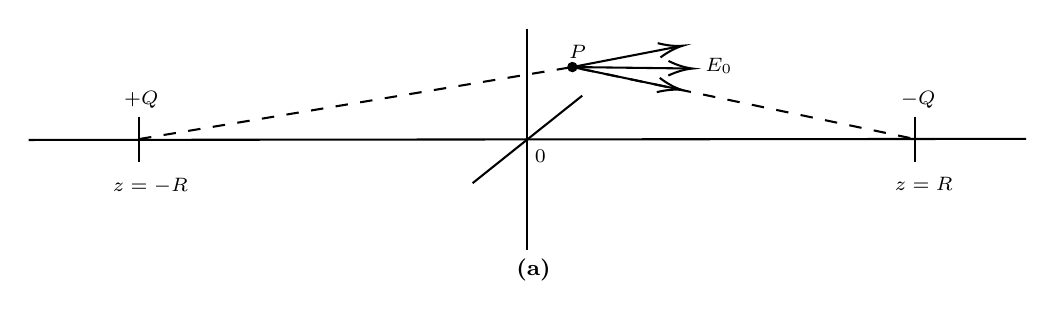
\begin{tikzpicture}[x=0.80pt,y=0.80pt,yscale=-1,xscale=1]
%uncomment if require: \path (0,300); %set diagram left start at 0, and has height of 300

%Straight Lines [id:da387033039470997] 
\draw    (100.17,150.67) -- (550.67,150.17) ;
%Straight Lines [id:da4119950680408605] 
\draw    (325.42,100.42) -- (325.42,200.42) ;
%Straight Lines [id:da9453033530891906] 
\draw    (350.17,130.67) -- (300.67,170.17) ;
%Straight Lines [id:da9447646112880248] 
\draw    (150,140.11) -- (150,160.44) ;
%Straight Lines [id:da6400000661091609] 
\draw    (500.5,140.11) -- (500.5,160.44) ;
%Straight Lines [id:da3090691549375759] 
\draw  [dash pattern={on 4.5pt off 4.5pt}]  (150,150.27) -- (345.73,117.73) -- (500.5,150.27) ;
%Shape: Circle [id:dp42319052305950877] 
\draw  [fill={rgb, 255:red, 0; green, 0; blue, 0 }  ,fill opacity=1 ] (343.87,117.81) .. controls (343.91,118.84) and (344.78,119.64) .. (345.81,119.6) .. controls (346.84,119.56) and (347.64,118.69) .. (347.6,117.66) .. controls (347.56,116.63) and (346.69,115.83) .. (345.66,115.87) .. controls (344.63,115.91) and (343.83,116.78) .. (343.87,117.81) -- cycle ;
%Straight Lines [id:da6032483981549016] 
\draw    (345.73,117.73) -- (398.03,118.38) ;
\draw [shift={(400.03,118.41)}, rotate = 180.71] [color={rgb, 255:red, 0; green, 0; blue, 0 }  ][line width=0.75]    (10.93,-3.29) .. controls (6.95,-1.4) and (3.31,-0.3) .. (0,0) .. controls (3.31,0.3) and (6.95,1.4) .. (10.93,3.29)   ;
%Straight Lines [id:da8576383356510381] 
\draw    (345.73,117.73) -- (393.67,108.47) ;
\draw [shift={(395.63,108.09)}, rotate = 169.06] [color={rgb, 255:red, 0; green, 0; blue, 0 }  ][line width=0.75]    (10.93,-3.29) .. controls (6.95,-1.4) and (3.31,-0.3) .. (0,0) .. controls (3.31,0.3) and (6.95,1.4) .. (10.93,3.29)   ;
%Straight Lines [id:da9565247126930154] 
\draw    (345.73,117.73) -- (393.28,127.68) ;
\draw [shift={(395.23,128.09)}, rotate = 191.81] [color={rgb, 255:red, 0; green, 0; blue, 0 }  ][line width=0.75]    (10.93,-3.29) .. controls (6.95,-1.4) and (3.31,-0.3) .. (0,0) .. controls (3.31,0.3) and (6.95,1.4) .. (10.93,3.29)   ;

% Text Node
\draw (327.42,153.82) node [anchor=north west][inner sep=0.75pt]  [font=\scriptsize]  {$0$};
% Text Node
\draw (492.67,127.17) node [anchor=north west][inner sep=0.75pt]   [font=\scriptsize]  {$-Q$};
% Text Node
\draw (141.83,127.17) node [anchor=north west][inner sep=0.75pt]   [font=\scriptsize] {$+Q$};
% Text Node
\draw (136.83,166.34) node [anchor=north west][inner sep=0.75pt]   [font=\scriptsize] {$z=-R$};
% Text Node
\draw (490,166.17) node [anchor=north west][inner sep=0.75pt]   [font=\scriptsize] {$z=R$};
% Text Node
\draw (319,203.07) node [anchor=north west][inner sep=0.75pt]  [font=\footnotesize] [align=left] {{\footnotesize \textbf{(a)}}};
% Text Node
\draw (342.83,106.34) node [anchor=north west][inner sep=0.75pt]   [font=\scriptsize] {$P$};
% Text Node
\draw (404.4,112.23) node [anchor=north west][inner sep=0.75pt]  [font=\scriptsize]  {$E_{0}$};


\end{tikzpicture}
\begin{tikzpicture}[x=0.80pt,y=0.80pt,yscale=-1,xscale=1]
%uncomment if require: \path (0,300); %set diagram left start at 0, and has height of 300

%Straight Lines [id:da14852568462004956] 
\draw    (98.67,150.33) -- (551.9,150.4) ;
%Shape: Circle [id:dp796137081820352] 
\draw   (259.49,150.37) .. controls (259.49,114.03) and (288.95,84.57) .. (325.28,84.57) .. controls (361.62,84.57) and (391.08,114.03) .. (391.08,150.37) .. controls (391.08,186.7) and (361.62,216.16) .. (325.28,216.16) .. controls (288.95,216.16) and (259.49,186.7) .. (259.49,150.37) -- cycle ;
%Shape: Circle [id:dp4481734607064437] 
\draw  [fill={rgb, 255:red, 0; green, 0; blue, 0 }  ,fill opacity=1 ] (293.24,150.24) .. controls (293.29,151.27) and (294.15,152.07) .. (295.18,152.03) .. controls (296.21,151.98) and (297.01,151.12) .. (296.97,150.09) .. controls (296.93,149.06) and (296.06,148.26) .. (295.03,148.3) .. controls (294,148.34) and (293.2,149.21) .. (293.24,150.24) -- cycle ;
%Straight Lines [id:da8667081935725879] 
\draw    (325.28,150.37) -- (362.25,201.84) ;
\draw [shift={(364,204.27)}, rotate = 234.31] [fill={rgb, 255:red, 0; green, 0; blue, 0 }  ][line width=0.08]  [draw opacity=0] (8.93,-4.29) -- (0,0) -- (8.93,4.29) -- cycle    ;
%Shape: Circle [id:dp07164027372366122] 
\draw  [fill={rgb, 255:red, 0; green, 0; blue, 0 }  ,fill opacity=1 ] (354.58,150.24) .. controls (354.62,151.27) and (355.49,152.07) .. (356.52,152.03) .. controls (357.55,151.98) and (358.35,151.12) .. (358.3,150.09) .. controls (358.26,149.06) and (357.39,148.26) .. (356.36,148.3) .. controls (355.33,148.34) and (354.53,149.21) .. (354.58,150.24) -- cycle ;
%Straight Lines [id:da5672292025283225] 
\draw    (150,139.61) -- (150,159.94) ;
%Straight Lines [id:da47992721458970344] 
\draw    (500.33,140.27) -- (500.33,160.61) ;
%Shape: Circle [id:dp3794070148151] 
\draw  [fill={rgb, 255:red, 0; green, 0; blue, 0 }  ,fill opacity=1 ] (421.58,57.57) .. controls (421.62,58.6) and (422.49,59.4) .. (423.52,59.36) .. controls (424.55,59.32) and (425.35,58.45) .. (425.3,57.42) .. controls (425.26,56.39) and (424.39,55.59) .. (423.36,55.63) .. controls (422.33,55.67) and (421.53,56.54) .. (421.58,57.57) -- cycle ;
%Straight Lines [id:da4463376085345808] 
\draw [color={rgb, 255:red, 0; green, 90; blue, 190 }  ,draw opacity=1 ]   (325.28,150.37) -- (367.25,110.43) -- (419.22,60.98) ;
\draw [shift={(420.67,59.61)}, rotate = 136.42] [color={rgb, 255:red, 0; green, 90; blue, 190 }  ,draw opacity=1 ][line width=0.75]    (10.93,-3.29) .. controls (6.95,-1.4) and (3.31,-0.3) .. (0,0) .. controls (3.31,0.3) and (6.95,1.4) .. (10.93,3.29)   ;
%Curve Lines [id:da7715951678163692] 
\draw    (405.67,149.94) .. controls (405.34,122.48) and (402.48,114.34) .. (386.58,96.03) ;
\draw [shift={(385.33,94.61)}, rotate = 48.67] [color={rgb, 255:red, 0; green, 0; blue, 0 }  ][line width=0.75]    (10.93,-3.29) .. controls (6.95,-1.4) and (3.31,-0.3) .. (0,0) .. controls (3.31,0.3) and (6.95,1.4) .. (10.93,3.29)   ;

% Text Node
\draw (335.33,178.27) node [anchor=north west][inner sep=0.75pt]  [font=\scriptsize][align=left] {a};
% Text Node
\draw (342.33,157.01) node [anchor=north west][inner sep=0.75pt]  [font=\scriptsize]  {$z=\ \dfrac{a^{2}}{R}$};
% Text Node
\draw (279.67,155.34) node [anchor=north west][inner sep=0.75pt]  [font=\scriptsize]  {$z=-\dfrac{a^{2}}{R}$};
% Text Node
\draw (143.33,126.67) node [anchor=north west][inner sep=0.75pt]  [font=\scriptsize]  {$+Q$};
% Text Node
\draw (492.67,126.67) node [anchor=north west][inner sep=0.75pt]  [font=\scriptsize] {$-Q$};
% Text Node
\draw (427.33,47.34) node [anchor=north west][inner sep=0.75pt]  [font=\scriptsize] {$P$};
% Text Node
\draw (136.33,167.34) node [anchor=north west][inner sep=0.75pt]  [font=\scriptsize]  {$z=-R$};
% Text Node
\draw (489,166.67) node [anchor=north west][inner sep=0.75pt]  [font=\scriptsize] {$z=R$};
% Text Node
\draw (358.33,100.67) node [anchor=north west][inner sep=0.75pt]  [font=\scriptsize]  {$r$};
% Text Node
\draw (406,115.01) node [anchor=north west][inner sep=0.75pt]  [font=\scriptsize]  {$\theta $};
% Text Node
\draw (287.5,125.9) node [anchor=north west][inner sep=0.75pt]  [font=\scriptsize]  {$\dfrac{aQ}{R}$};
% Text Node
\draw (345,126.4) node [anchor=north west][inner sep=0.75pt]  [font=\scriptsize]  {$-\dfrac{aQ}{R}$};

\draw (319,220) node [anchor=north west][inner sep=0.75pt]  [font=\footnotesize] [align=left] {{\footnotesize \textbf{(b)}}};
\end{tikzpicture}
\caption{Düzgün elektrik alanında iletken küre problemininin görüntü yükleri yöntemiyle çözümü.}
\end{figure}
\begin{align*}
\phi(a) =  0 
\end{align*}
\begin{align*}
\phi(\vec{r}) = \dfrac{1}{4 \pi \varepsilon_{0}} \Bigg\{ \dfrac{Q}{|\vec{r} + \vec{R}|} + \dfrac{-Q}{|\vec{r}- \vec{R}|}  +\dfrac{q}{|\vec{r}- \vec{R'}|} + \dfrac{-q}{|\vec{r} + \vec{R'}|} \Bigg\}
\end{align*}
\begin{align*}
= k\Bigg\{ \dfrac{Q}{|\vec{r} + \vec{R}|} + \dfrac{-Q}{|\vec{r}- \vec{R}|}  +\dfrac{aQ}{R |\vec{r}- \dfrac{a^{2}}{R^{2}}\vec{R'}|} + \dfrac{-aQ}{R |\vec{r} + \dfrac{a^{2}}{R^{2}} \vec{R'}|} \Bigg\}
\end{align*}

Orijinal problemin $\phi (a) =  0 $ sınır koşulu sağlanır.

\begin{align*}
    = kQ \Bigg\{ \dfrac{1}{|\vec{r} + \vec{R}|} - \dfrac{1}{|\vec{r} - \vec{R}|} \Bigg\} + \dfrac{aQ}{R} k \Bigg\{ \dfrac{1}{|\vec{r} - \dfrac{a^{2}}{R^{2}} \vec{R}|} - \dfrac{1}{|\vec{r} + \dfrac{a^{2}}{R^{2}} \vec{R}|} \Bigg\}
\end{align*}

$\vec{r}$ ve $\vec{R}$ arasındaki açı $\theta$'dır.

\begin{align*}
\phi(\vec{r}) &= \kQ \Bigg\{ \dfrac{1}{[ r^{2} + R^{2} + 2Rr \cos \theta]^{1/2}} - \dfrac{1}{[ r^{2} + R^{2} - 2Rr \cos \theta]^{1/2}} \Bigg\} \\ 
&+ \dfrac{aQ}{R} k  \Bigg\{ \dfrac{1}{ \Big[ r^{2} + R^{2}  \dfrac{a^{4}}{R^{4}} - 2r \dfrac{a^{2}}{R^{2}} R \cos \theta \Big]^{1/2}} - \dfrac{1}{ \Big[ r^{2} + R^{2}   \dfrac{a^{4}}{R^{4}} + 2r \dfrac{a^{2}}{R^{2}} R \cos \theta \Big]^{1/2}} \Bigg\} 
\end{align*}

\end{theorem}
\section{Problemler}